% general format definition
\documentclass[a4paper, 11pt]{article}
\usepackage[margin=.9in]{geometry}
\usepackage[utf8]{inputenc}
\usepackage[T1]{fontenc}
\usepackage[english]{babel}

% extra packages
\usepackage{hyperref}
\usepackage{listings}
\usepackage{color}
\usepackage{amssymb}
\usepackage{amsmath}
\usepackage{mathtools}
\usepackage{microtype}
\usepackage{stmaryrd}
\usepackage{tikz}
\usetikzlibrary{arrows,automata,positioning}


% special math symbols
\newcommand{\R}{\ensuremath{\mathbb{R}}}
\newcommand{\N}{\ensuremath{\mathbb{N}}}
\newcommand{\Z}{\ensuremath{\mathbb{Z}}}
\newcommand{\Q}{\ensuremath{\mathbb{Q}}}

% Syntax highlighting
\definecolor{commentsColor}{rgb}{0.497495, 0.497587, 0.497464}
\definecolor{keywordsColor}{rgb}{0.000000, 0.000000, 0.635294}
\definecolor{stringColor}{rgb}{0.558215, 0.000000, 0.135316}
\lstset{
  backgroundcolor=\color{white},                        % choose the background color; you must add \usepackage{color} or \usepackage{xcolor}
  basicstyle=\footnotesize,                             % the size of the fonts that are used for the code
  breakatwhitespace=false,                              % sets if automatic breaks should only happen at whitespace
  breaklines=true,                                      % sets automatic line breaking
  captionpos=b,                                         % sets the caption-position to bottom
  commentstyle=\color{commentsColor}\textit,            % comment style
  deletekeywords={},                                    % if you want to delete keywords from the given language
  escapeinside={\%*}{*)},                               % if you want to add LaTeX within your code
  extendedchars=true,                                   % lets you use non-ASCII characters; for 8-bits encodings only, does not work with UTF-8
  frame=tb,	                   	                        % adds a frame around the code
  keepspaces=true,                                      % keeps spaces in text, useful for keeping indentation of code (possibly needs columns=flexible)
  keywordstyle=\color{keywordsColor}\bfseries,          % keyword style
  otherkeywords={True,False,true,false,null,None,NULL}, % if you want to add more keywords to the set
  numbers=left,                                         % where to put the line-numbers; possible values are (none, left, right)
  numbersep=5pt,                                        % how far the line-numbers are from the code
  numberstyle=\tiny\color{commentsColor},               % the style that is used for the line-numbers
  rulecolor=\color{black},                              % if not set, the frame-color may be changed on line-breaks within not-black text (e.g. comments (green here))
  showspaces=false,                                     % show spaces everywhere adding particular underscores; it overrides 'showstringspaces'
  showstringspaces=false,                               % underline spaces within strings only
  showtabs=false,                                       % show tabs within strings adding particular underscores
  stepnumber=1,                                         % the step between two line-numbers. If it's 1, each line will be numbered
  stringstyle=\color{stringColor},                      % string literal style
  tabsize=2,	                                          % sets default tabsize to 2 spaces
  title=\lstname,                                       % show the filename of files included with \lstinputlisting; also try caption instead of title
  columns=fixed,                                        % Using fixed column width (for e.g. nice alignment)
}

\author{Thilo Metzlaff\\406247 \and Mats Frenk\\393702\and René van Emelen\\406008}
\title{FoSAP Exercise 4 \\ \large Group 3}
\begin{document}
    % titlepage
    \maketitle
    \newpage

    % contents
    \tableofcontents
    \newpage

    % section 0
    \section*{Introduction}
    Welcome To this special endeavour, where i write every single thing in \LaTeX{}
    How is any of this gonna work?\\
    Simple: With patience and a format definition. Therefore, please let me define the format of this.

    \subsection*{THE FORMAT}
    \begin{itemize}
        \item Every file will be named similar to the sections in here, so\\
              \texttt{2.1-stack\_exercise.c} is Exercise 2, section 1.
        \item Every Solution \textbf{WILL} be in this pdf, but not necessarily 
              anything predefined by the exercise.
        \item Any explanation will be both in this PDF as well as in each file.
        \item This explanation will be in each PDF, in case someone who doesn't
              know the format tries to correct the exercises
    \end{itemize}
    \newpage
    \begin{figure}[h]
      \centering
      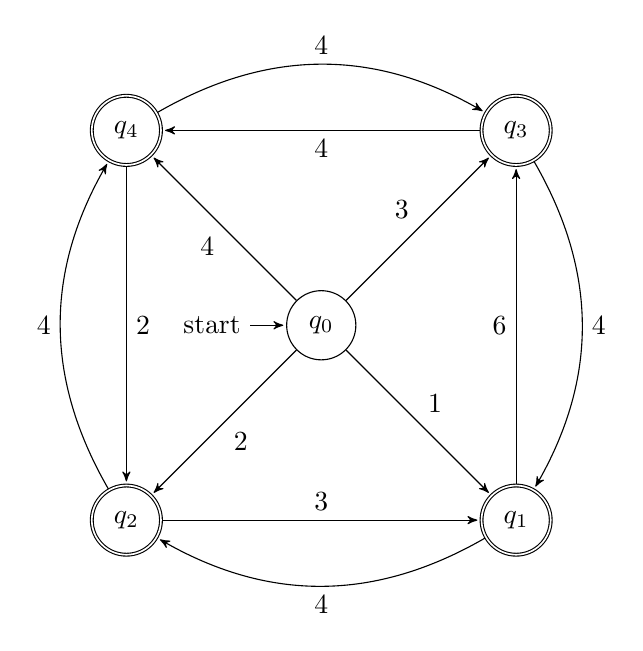
\begin{tikzpicture}[->,>=stealth',shorten >=1pt,auto,node distance=3.5cm,
            scale = 1,transform shape]
      
            \node[state,initial] (q_0) {$q_0$};
            \node[state,accepting] (q_1) [below right of=q_0] {$q_1$};
            \node[state,accepting] (q_2) [below left of=q_0] {$q_2$};
            \node[state,accepting] (q_3) [above right of=q_0] {$q_3$};
            \node[state,accepting] (q_4) [above left of=q_0] {$q_4$};
      
      
            \path (q_0) edge              node {$1$} (q_1)
                  (q_0) edge              node {$2$} (q_2)
                  (q_0) edge              node {$3$} (q_3)
                  (q_0) edge              node {$4$} (q_4)
      
                  (q_1) edge [bend left]  node {$4$} (q_2)
                  (q_2) edge [bend left]  node {$4$} (q_4)
                  (q_3) edge [bend left]  node {$4$} (q_1)
                  (q_4) edge [bend left]  node {$4$} (q_3)
      
                  (q_4) edge              node {$2$} (q_2)
                  (q_2) edge              node {$3$} (q_1)
                  (q_3) edge              node {$4$} (q_4)
                  (q_1) edge              node {$6$} (q_3)
                  ;
      
         \end{tikzpicture}
         \caption[sd]{Test}
    \end{figure}
\end{document}